%% Utku: Hey folks, I'm going to add comments here that I want to keep in context so that I can get your input and just discuss in-place instead of Zulip. 
% 
% I'm trying to lead the introduction part in the direction of the narrative
% that FinStoch and Stoch are the prototypical categories for the concept of a
% Markov category, and so the eventual definition of a Markov category that
% we'll reach is motivated by the inherent structure present in these two
% categories.
%
% Check my TODOs for my plans etc.
%

\subsection{Informal introduction to Markov kernels and Markov categories}

\begin{frame}[c]
    A Markov category consists of
    \begin{enumerate}
        \item objects: spaces of possible states\par
            Alphabets or data
            Represented as wires
            % TODO?: Add wire diagram
        \item morphisms: channels, devices, programs
            We represent them as boxes to be read horizontally from left to right.
            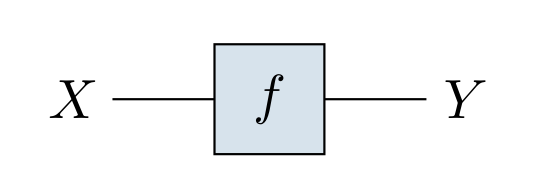
\includegraphics[width=.4\textwidth]{graphics/string/markov_morphism.png}
    \end{enumerate}
    Morphisms are in general \emph{noisy}, involving randomness
\end{frame}

\begin{frame}
    \frametitle{Prototypical Markov categories}
    % Should this really be its own frame?
    \begin{enumerate}
        \item FinStoch: 
            \begin{itemize}
                \item objects: finite alphabets $X, Y, \dots$
                \item morphisms: stochastic matrices $f: X\to Y$
            \end{itemize}
        \item Stoch: 
            \begin{itemize}
                \item objects: measurable sets/alphabets $(X, \Sigma_X), Y\ \text{(when clear from context)}, \dots$
                \item morphisms: Markov kernels $f: X\to Y$
            \end{itemize}
    \end{enumerate}
\end{frame}

\begin{frame}
    \frametitle{FinStoch}
    \framesubtitle{What are Stochastic matrices?}
    \begin{minipage}{.48\textwidth}
        A stochastic matrix from alphabet $X$ to alphabet $Y$ is a matrix of non-negative entries
        \begin{align*}
            X\times Y \to [0,1]\\
            (x, y) \mapsto f(y\mid x)
        \end{align*}
        such that each column sums to one:
        \[
            \sum_{y\in Y} f(y\mid x) = 1 \quad \text{for every $x\in X$.}
        \]
    \end{minipage}
    \hfill
    \begin{minipage}{.48\textwidth}
        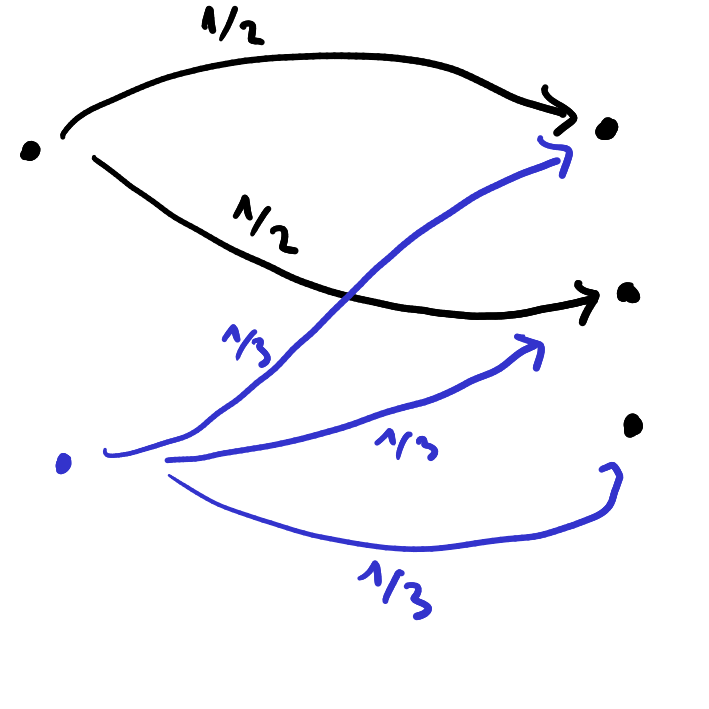
\includegraphics[width=\textwidth]{finstoch_mkv_kernel}
    \end{minipage}
\end{frame}

\begin{frame}
    \frametitle{Stoch}
    \framesubtitle{What are measurable spaces and Markov kernels?}
    % TODO?: do we talk about $\sigma$-algebras in detail
    A Markov kernel from measurable space $(X, \Sigma_X)$ to $(Y, \Sigma_Y)$ is an assignment
    \begin{align*}
        X\times \Sigma_Y \to [0, 1]\\
        (x, S) \mapsto f(S\mid x)
    \end{align*}
    which is measurable in $X$ and is a probability measure in $Y$.
\end{frame}

\begin{frame}
    For both examples, we can equivalently see the channels $X\to Y$ as (measurable) functions $X\to PY$, where for $x\in X$, $f_x$ is a probability measure of $Y$.

    % TODO: a short mention of probability monads here
    
\end{frame}

\subsection{Markov categories are categories}

\begin{frame}
    \frametitle{Identity}
    \framesubtitle{through Dirac delta distribution}
    % TODO: Shorten this frame
    The fact that we have a category means the following. First of all, we have an identity morphism $1_X: X\to X$ for each object (alphabet) $X$, which represents no change in the state of $X$. We draw it simply with a wire
    In FinStoch, identities are identity matrices. In Stoch, they are the "Dirac delta" kernels defined by the identity function
    \[
        \text{\normalfont id} (S\mid x) = \delta_x (S) = 1_S(x) = \begin{cases} 1\ x\in S\\ 0\ x\not \in S
        \end{cases}
    \]
\end{frame}

\begin{frame}
    \frametitle{Composition}
    \framesubtitle{through the Chapman-Kolmogorov equation}
    % TODO: Shorten this frame
    % Composition (Stoch, FinStoch) through the Chapman-Kolmogorov equation (measure pushfwd, matmul)
    Moreover, we have a notion of sequential composition of channels: given channels f : X → Y and g : Y → Z, we can form a channel g ◦ f : X → Z, which we draw as follows.
    In FinStoch the composition is given by the \emph{Chapman-Kolmogorov} formula:
    \begin{align}
        g\circ f (z\mid x) \coloneqq \sum_{y\in Y} g(z\mid y) f(y\mid x)
    \end{align}
    and in Stoch it is given by its continuous analogue: for every measurable subset $S\subset Z$,
    \begin{align}
        g\circ f (S\mid x) \coloneqq \int_Y g(S\mid y) f(dy\mid x)
    \end{align}
    by which we mean the integral with respect to the measure $f_x$ on $Y$, for every $x$.
\end{frame}

\begin{frame}
    \frametitle{A basic example for $\mathsf{FinStoch}$}
    \begin{minipage}{.48\textwidth}
    The \emph{Chapman-Kolmogorov} formula:
    \begin{align*}
        g\circ f (z\mid x) \coloneqq \sum_{y\in Y} g(z\mid y) f(y\mid x)
    \end{align*}
    \end{minipage}
    \hfill
    \begin{minipage}{.45\textwidth}
        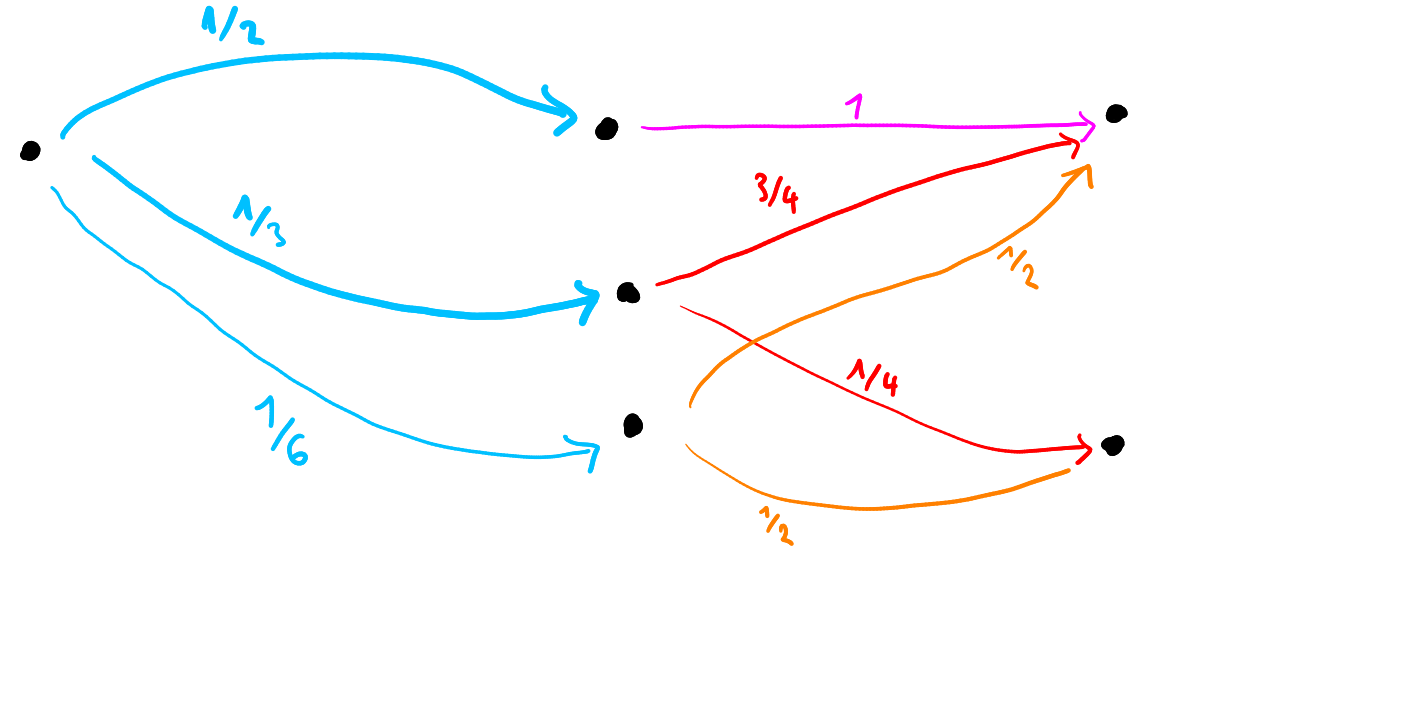
\includegraphics[width=\textwidth]{finstoch_matmul.png}
        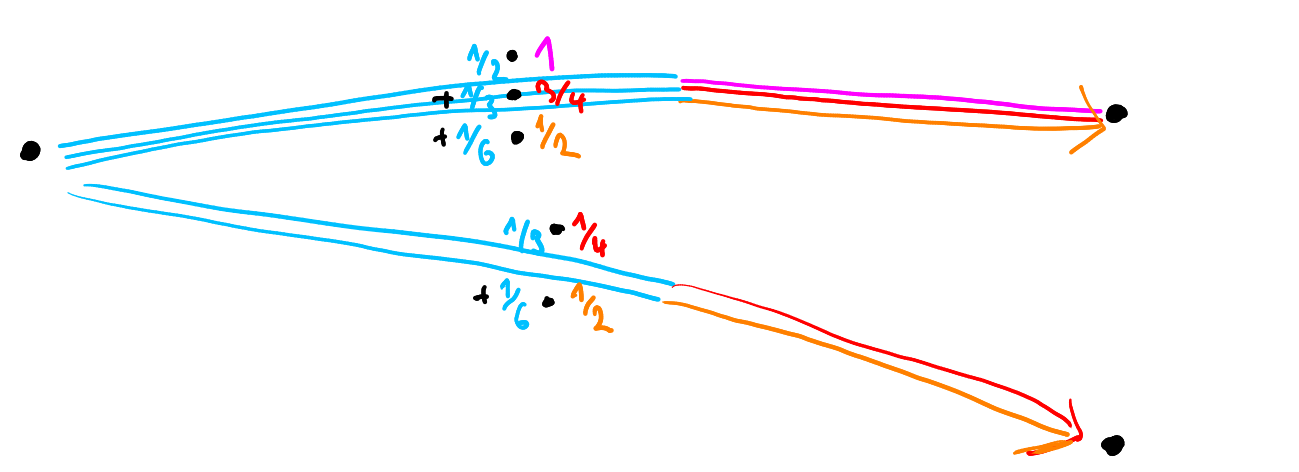
\includegraphics[width=\textwidth]{finstoch_matmul_2.png}
    \end{minipage}
    
\end{frame}

\subsection{Markov categories are symmetric monoidal}
\begin{frame}
    \frametitle{States}
    \framesubtitle{form probability distributions}
    % States form probability distributions
    % TODO: Rephrase to simplify what a source is in Fin/Stoch and what it should be in a MC
unit we write $I$, and which we do not draw (it’s represented by an empty region). 

In FinStoch and Stoch it is the one-point space, where there is no distinction between states to be made.

A source, or (random) state on X is now a morphism $p: I\to X$, which we depict as follows.
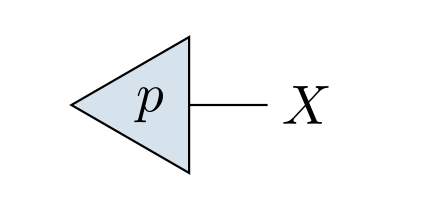
\includegraphics[width=.4\textwidth]{graphics/string/markov_state.png}

(mass fnc for FinStoch??)
\begin{enumerate}
    \item FinStoch: a source is a stochastic "column" matrix, a finite probability measure on $X$
    \item Stoch: A Markov kernel to X with no input, i.e. a probability measure on $X$
\end{enumerate}

\end{frame}

\begin{frame}
    \frametitle{Parallel composition} 
    \framesubtitle{is "independent"}
Markov categories also come with a notion of parallel composition. $X\otimes A$, and which we interpret as the object whose states are composite states. in FinStoch and in Stoch it is given by the cartesian product of measurable spaces. Now given channels $f: X\to Y$ and $h: A\to B$, we can form the tensor product channel $f\otimes h: X\otimes A\to Y\otimes B$, which we represent as follows
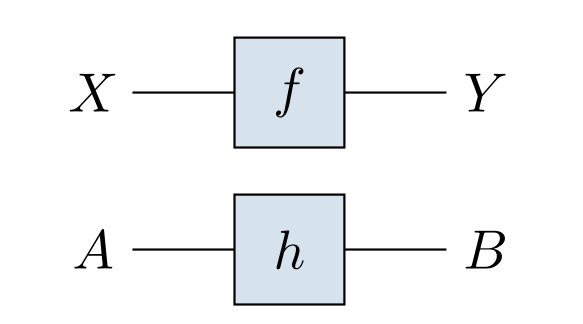
\includegraphics[width=.4\textwidth]{graphics/string/markov_parallel.png}
and which we interpret as processing X and A independently. Compare this with a generic channel $g: X\otimes A\to Y\otimes B$
% TODO?: <include a generic two-input-output channel here>
where for example, Y can possibly depend on both X and A. In FinStoch, the tensor product of the stochastic matrices f : X → Y and g : A → B is given by the product of the individual entries,
\[
    f\otimes h(y, b\mid x, a)\coloneqq f(y\mid x)h(b\mid a)
\]
\end{frame}

\begin{frame}
    \begin{center}
        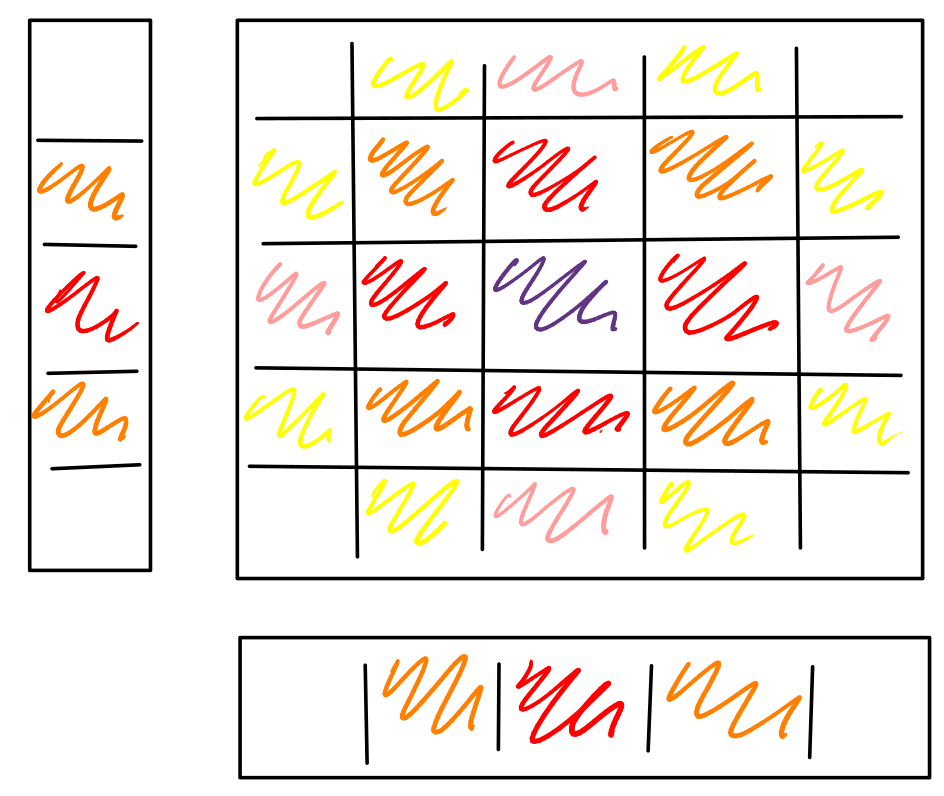
\includegraphics[width=.7\textwidth]{finstoch_parallel_composition.png}
    \end{center}
\end{frame}

\subsection{Markov categories have comonoid objects}
\begin{frame}
    \frametitle{copy structure}
    \begin{minipage}{.55\textwidth}
        The last piece of structure that we need to form a Markov category is two distinguished maps for each object X: a map $\text{\normalfont copy}: X\to X\otimes X$ which we call “copy” or “duplicate”, and represent as follows
        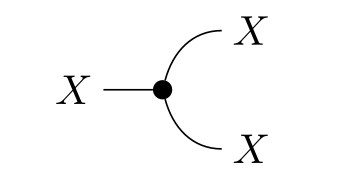
\includegraphics[width=.4\textwidth]{graphics/string/markov_copy.png}
    \end{minipage}
    \hfill
    \begin{minipage}{.4\textwidth}
        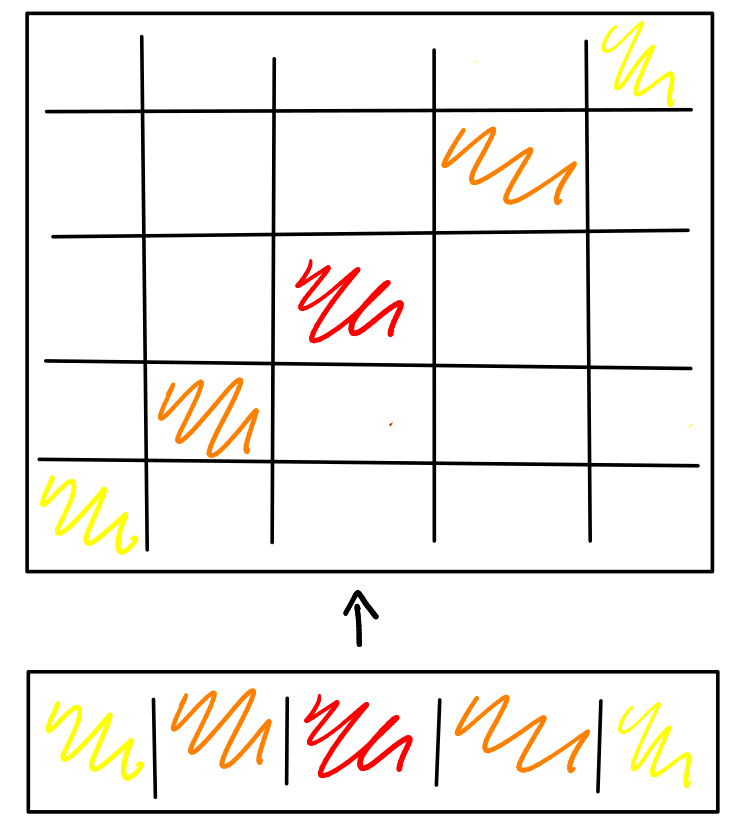
\includegraphics[width=\textwidth]{copy_graphic}
    \end{minipage}
\end{frame}


\begin{frame}
    \frametitle{delete structure}
    \begin{minipage}{.48\textwidth}
        Short intuitive description
        % TODO?: <add the delete string diagram here>
    \end{minipage}
    \hfill
    \begin{minipage}{.48\textwidth}
        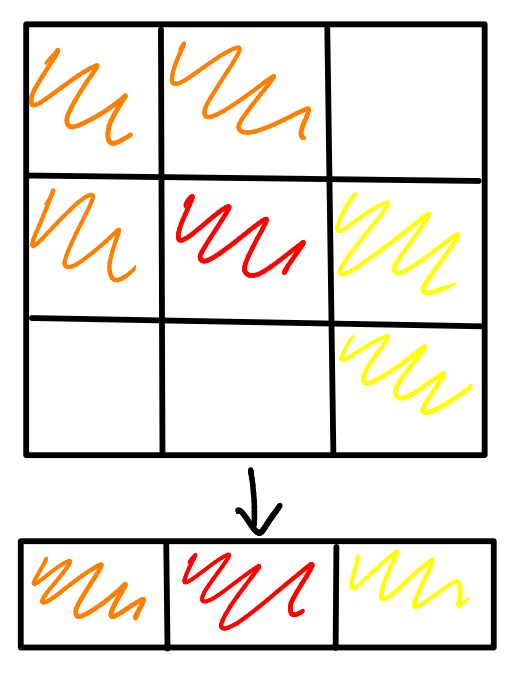
\includegraphics[width=\textwidth]{delete_graphic.png}
    \end{minipage}
\end{frame}

\begin{frame}[t]
    \frametitle{Marginals}
    \framesubtitle{from copy and delete}
    Marginals, colorful picture for finstoch: “If you have the tensor product and delete morphism, then marginals come automatically for free. No more integrating over variables!”
\end{frame}

\begin{frame}
    \frametitle{Naturality of delete}
The last property that we require in a Markov category is normalization or counitality: applying a morphism f and discarding its output is the same as discarding the input from the start.  In FinStoch, this is exactly the condition that the sum of each column of a stochastic matrix is one, i.e. that transition probabilities are normalized.
% TODO: loop back to when we talked about normalization and say that naturality of delete suffices to reflect this
\end{frame}

\subsection{Formal definition of Markov categories}

\begin{frame}
    % “A Markov category is a semicartesian category where all objects are commutative comonoids compatible with the monoidal structure”
    \begin{definition}
        A Markov category is a symmetric monoidal category $(\mathsf{C}, \otimes, I)$ together with a chosen commutative comonoid structure for each object $X$, which is compatible with tensor products, and for which all morphisms are counital.
    \end{definition}
    \begin{minipage}{.48\textwidth}
        \begin{enumerate}
            % minipages for each item??
            \item $\mathsf{C}$ is semi-cartesian
            \item Each object $X$ is equipped with "copy" and "discard" maps
            \item which satisfy the identities of a commutative monoid
            \item The copy maps are compatible with the monoidal structure in the following way
        \end{enumerate}
    \end{minipage}
    \hfill
    \begin{minipage}{.48\textwidth}
        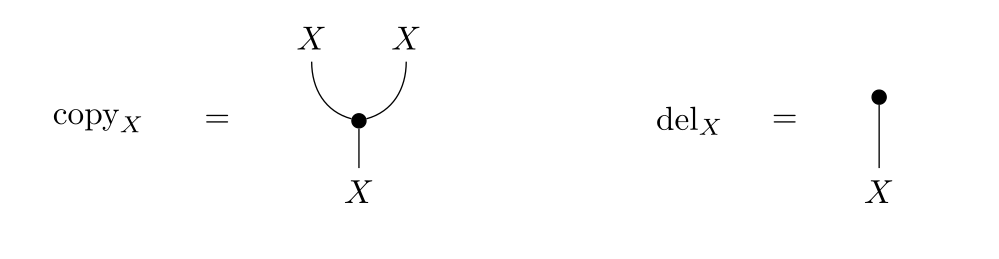
\includegraphics[width=\textwidth]{graphics/string/markov_copy_delete.png}
        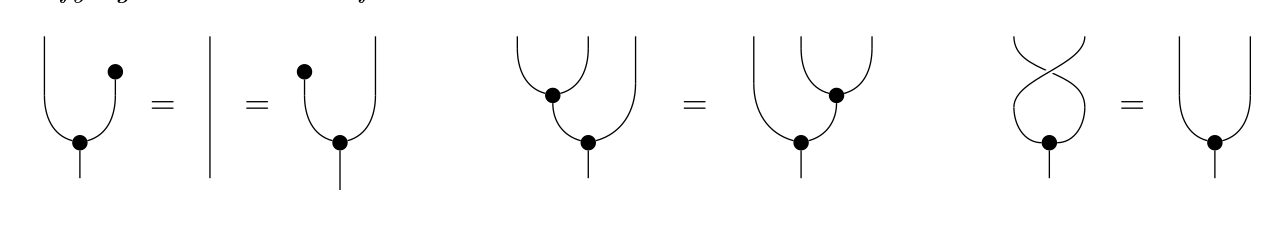
\includegraphics[width=\textwidth]{graphics/string/markov_commutative_monoid.png}
        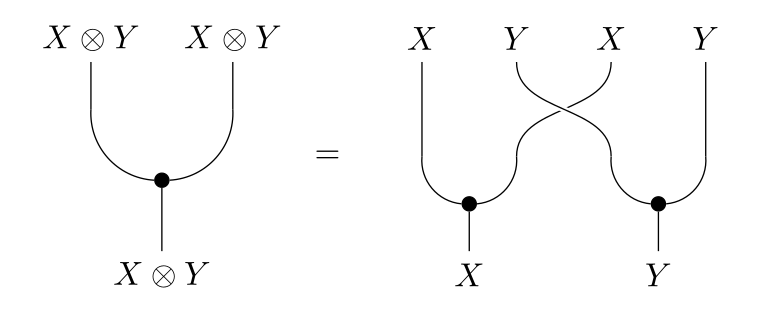
\includegraphics[width=\textwidth]{graphics/string/markov_monoidal_compat.png}
    \end{minipage}
\end{frame}

\begin{frame}
    % Do we need to mention that Markov categories admit string diagrams? Can we just mention it offhand and get it over with then?
    quick mention that Markov categories admit string diagrams
\end{frame}
